% 必要な項目ができた場合は適宜サブセクションを追加してください
%使用するパッケージ

%\include{begin}

\documentclass[a4j,titlepage]{jarticle}
\usepackage[dvipdfmx]{graphicx,epsfig}

\usepackage{longtable}

\usepackage{textcomp}



\usepackage{float}

\usepackage{ascmac}
\usepackage{fancybox}
\usepackage{url}


\begin{document}
% イベント名を記入する
\section{積んで積んで積みまくれ! つむつむ(仮)}


% 日時と場所を記入する
% 時刻は4桁で記入すること!
\subsection{日時・場所}
\begin{tabular}{p{2zw}rp{38zw}}
  日時 & : & 2019年4月6日(土) 9:35 $\sim$ 10:28 \\
  場所 & : & つどいの広間
\end{tabular}


% 目的を記入する
\subsection{目的}
本イベントは新入生全員がチームをつくり,そのチームの仲間と協力して他のチームと競うことで,より交流を深めて貰うことを目的とする.班内のスタッフは随時新入生が全員映るような写真を撮る

% イベントの概要やルールを記入する
\subsection{イベント内容}
16班対抗で,大量に与えられた紙と本を用いてタワーを作る.ゲーム開始の合図とともに,タワーを作りはじめ,制限時間8分の間にポイントが高いタワーを作ることができるかを競うゲームである.1回目の作戦タイムの後にタワーを立て測定し,順位を発表する.その後,他の順位を参考に短めの作戦タイムを利用して1回目の作戦の反省と二回目に向けた作戦を立てる.二回目の作戦タイム終了後,タワーを作成し計測する.その際の得点は1回目の得点との合計をその班の得点とする.

\begin{enumerate}
\item チーム1から順に等間隔で並ぶ.(図\ref{fig:paper}参照)
\item 10分間の作戦タイムをとる.
\item 作戦タイム時,10枚の紙と本で練習してもらう.
\item ゲーム開始の合図で50枚の紙と3冊の本を用いて一斉にタワーを作り始める.制限時間は8分で,ゲーム終了の合図でタワーから手を放し,測定係(各班スタッフ)が測定を開始し,順位をつける.
\item 得点については,
  
  $(本1の得点)*(本1までの高さ[cm]) + (本2の得点)*(本2までの高さ[cm]) + (本3の得点)*(本3までの高さ[cm]) + タワーそのものの高さ[cm]) = (チームの得点)$
  
  とする.
\item 本の得点は,・・・・・・・
\item 5分間の作戦タイムをとる.
\item その後は1回目と同様にタワーを立てて計測する.
\item 全ての班の得点が出揃い次第総合順位を発表
\item 終了


\end{enumerate}

%\clearpage


% イベントのタイムスケジュールを記入する
% 時刻は必ず4桁(00:00)で記入すること!
% 時間の流れは途切れないように記述する!
\subsection{タイムスケジュール}
\begin{longtable}{p{3zw}p{39zw}}
  %10:20
  09:35 & \textbf{◎ つむつむ(仮)の準備} \\
  & \ \ \textbullet \ \  目安2分間で準備をする\\
        & \ \  \textbullet \ \ 休憩の間,各班のスタッフを筆頭にゲームの準備を行う\\
        & \ \  \textbullet \ \ 各チームのスタッフは$(紙10枚と紙50枚)*2$のまとまりを持っておく\\
        & \ \  \textbullet \ \ 総合司会者が所定の位置にチームを配置させる(図1参照)\\
        %& \ \  \textbullet \ \ デモプレイ係は司会側の脇に待機する\\\\

  %10:30
  09:37 & \textbf{◎ つむつむ(仮)の説明} \\
        & \ \ \textbullet \ \ 6分でゲームの説明を行う\\
        & \ \ \textbullet \ \ 総合司会がゲームのプレゼンターに司会権を振り,プレゼンターがゲームの全般の説明をする\\
  %10:35
  09:43 & \textbf{◎ 1回目の作戦タイム} \\
        & \ \ \textbullet \ \ 司会者が10分間の作戦タイムをとる\\
        & \ \ \ \ \ 班内のスタッフは随時新入生が全員映るような写真を撮る \\
        & \ \ \ \ \ (※10枚の紙を用いて練習をしてもらう) \\
        & \ \ \ \ \ (※この間,司会は実況する) \\
  %10:50
  09:53 & \textbf{◎ 1回目の作成タイム} \\
        & \ \ \textbullet \ \ 10分間たったら,司会者がゲームスタートの合図を出す\\
        & \ \ \textbullet \ \ 司会者はストップウォッチで8分を計測する\\
        & \ \ \ \ \ (※この8分間,司会者はそれぞれのチームの進行具合を実況する) \\
        & \ \ \textbullet \ \ 8分間たったら司会者はゲームをやめさせ,タワーから手を離すよう促す\\\\

  %11:00
  10:01 & \textbf{◎ 1回目の計測,結果,片付け} \\
        & \ \ \textbullet \ \ 各班のスタッフはタワーの高さを小数点以下切り捨てで計測し,得点を計算する.その後,前に集まり順位を出し,司会者に伝える \\
        & \ \ \ \ \ (※ミリは切り捨てで計測する) \\
        & \ \ \ \ \ (※測定中,司会者は間を持つように実況する) \\
        & \ \ \textbullet \ \ 各班のスタッフは元の班にかえる \\
        & \ \ \textbullet \ \ 司会者は3位$\sim$1位のスコアを口頭で発表する \\
        %& \ \ \textbullet \ \ 準備係が参加賞を参加者全員に配る\\
        %& \ \ \textbullet \ \ 準備係が1位と2位のチームに,優勝チーム賞,準優勝チーム賞をチームの人数分配る\\
        & \ \ \textbullet \ \ タワーを崩して紙を平らにしてもらうよう促す \\
        & \ \ \textbullet \ \ 平らにした紙は各班のスタッフが回収する \\
  10:08 & \textbf{◎ 2回目の作戦タイム} \\
        & \ \ \textbullet \ \ 司会者が5分間の作戦タイムをとる \\
        & \ \ \textbullet \ \ 1回目と同様に動いてもらう \\
  10:13 & \textbf{◎ 2回目の作成タイム} \\
        & \ \ \textbullet \ \ 5分間経ったら,司会者がゲームスタートの合図を出す\\
        & \ \ \textbullet \ \ 1回目と同様に動いてもらう \\
  10:21 & \textbf{◎ 2回目の計測,結果,片付け} \\
        & \ \ \textbullet \ \ 1回目と同様に計測 \\
        & \ \ \textbullet \ \ 2回目測定後,各班の総合得点が出揃い次第上位チームを表彰する.(賞品があれば授与する) \\
     & \ \ \textbullet \ \ 各班員とスタッフで協力して使用した紙等を片付ける \\
        & \ \ \textbullet \ \ 司会者がイベント終了の挨拶的なものをする \\\\
  %11:20
  10:28 & \textbf{◎ 終了し休憩(15分)} \\

\end{longtable}


% イベントに必要な役割と人数を記入する
% 担当者は決定次第追記する
% 記入例 ・司会者 2人(名前1,名前2)
\subsection{人員配置}
\begin{itemize}
\item 司会:横田,長通
\item プレゼンター:藤田(竜世),生野
\item 測定係:各班のスタッフ
\item 機器操作:和田
\end{itemize}


% イベントを実施するときに新入生や先生,スタッフがどこに配置するかを記入する
% 図があるとわかりやすい
\subsection{全体配置}
\begin{figure}[h]
  \begin{center}
    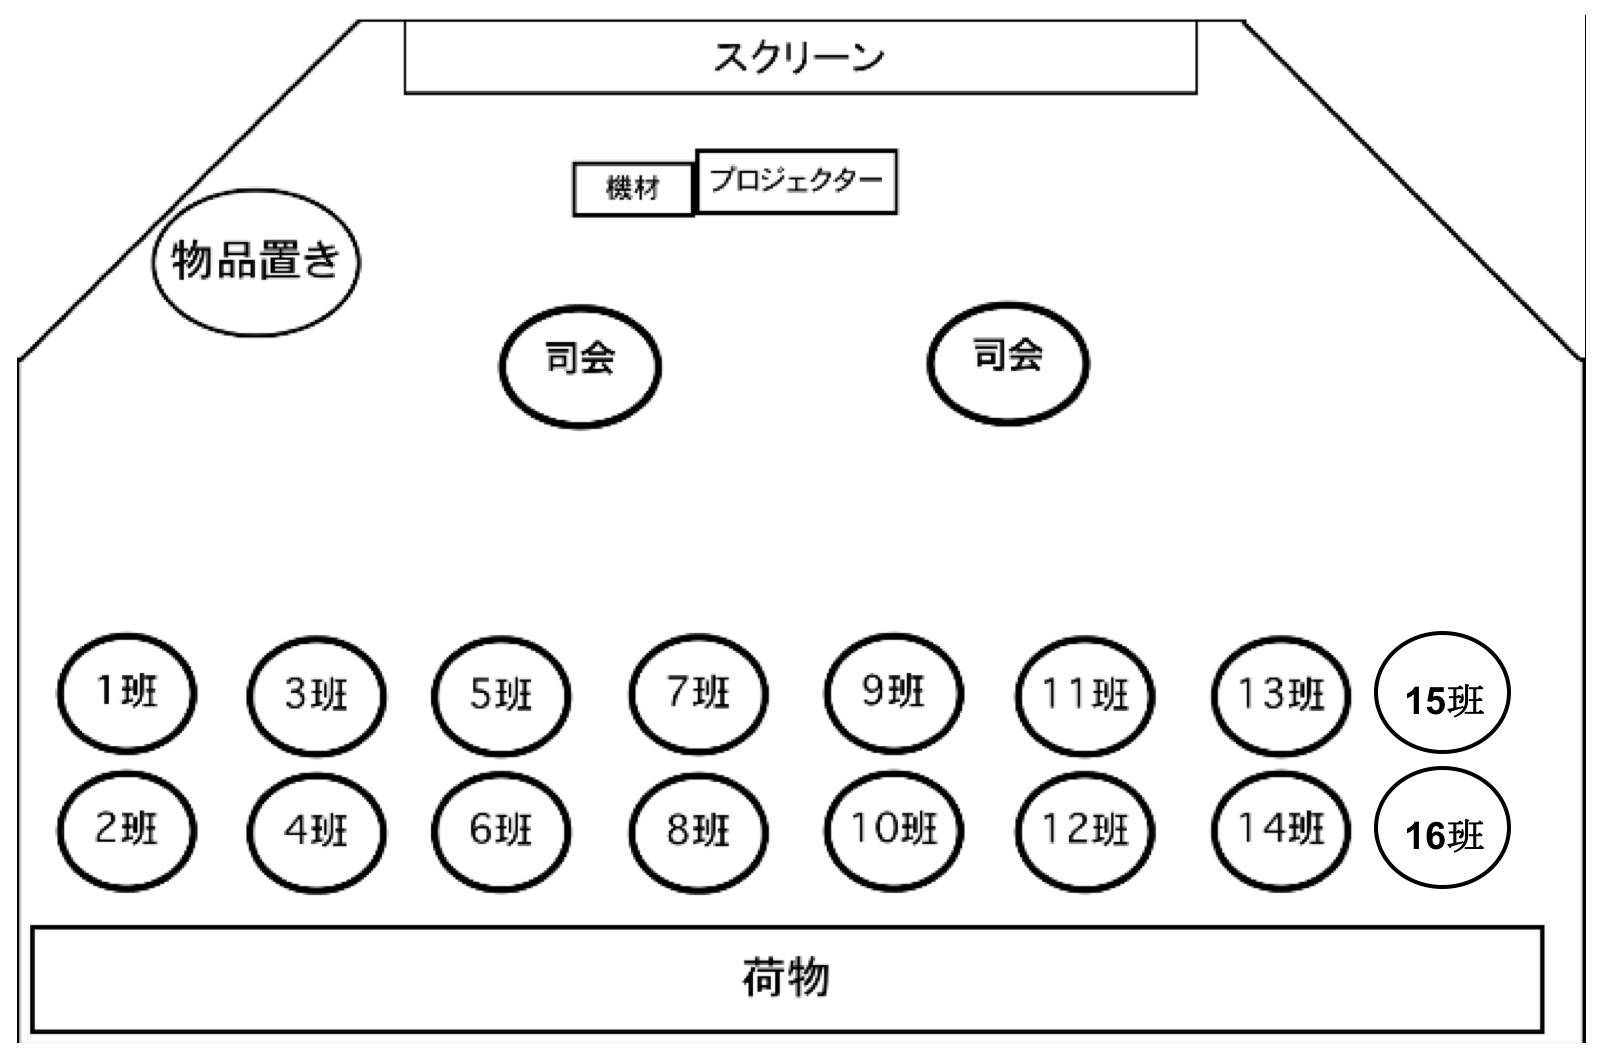
\includegraphics[scale=0.5]{./22/ice.eps}
    \caption{つむつむ(仮)の配置}
    \label{fig:paper}
  \end{center}
\end{figure}

% イベントに必要な物品と個数を記入する
% 記入例 ・マジックペン 10本
\subsection{必要物品}
\begin{itemize}
\item マイク:2本
\item スピーカー:2つ
\item 測定用のメジャー:14コ
\item 紙 : 1920枚${16(チーム)×{10枚(作戦タイム用)+50(本番用)}*2}$
\item 予備の紙 : 100枚 (予備)
\item 60枚の紙を入れるクリアファイル:32枚
\item スクリーン:1つ
\item プロジェクター:1つ
\item カメラ:1つ
\item 本:56冊 {16(チーム)×3(冊) + 予備8(冊)}
%\item 参加賞(うまい棒):人数分
%\item 優勝チーム賞(ビックカツ):優勝チームの人数分
%\item 準優勝チーム賞(チロルチョコ):準優勝チームの人数分
\end{itemize}


% 注意事項やスタッフに周知しておくべきことがあれば記入する
\subsection{備考}
\begin{itemize}
\item なるべく時間通りに進め,時間をオーバーしている場合は司会者は進行を速め,時間が余っている場合は時間をトークでかせぐようにするのが望ましい
\item ルールが分からない人が出てくるので,分からなそうな人がいたら声をかけてあげるとよい
\end{itemize}

%\include{end}


% --*- coding:utf-8-unix mode:latex -*--
% Endファイル

\end{document}
